\hypertarget{section-building-block-view}{%
\section{Building Block View}\label{section-building-block-view}}
In this chapter, we present the building block view of our application, illustrating how each component is structured and integrated within the system. The aim is to provide a comprehensive overview of the major software building blocks, focusing on their responsibilities and interactions.
\subsection{System White Box}
\begin{figure}[H]
    \centering
    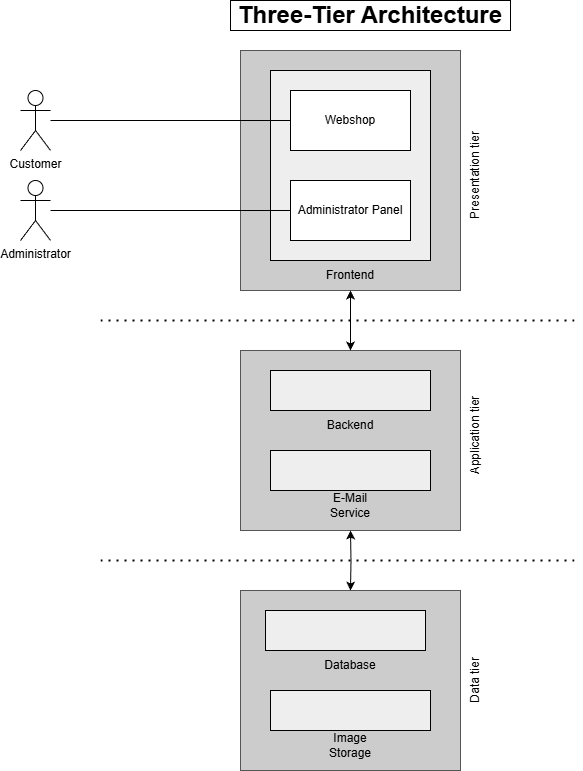
\includegraphics[width=0.8\textwidth]{images/building_block_system_whitebox.png}
    \caption{Whie Box View of the System}
\end{figure}

\subsubsection{Motivation}
We utilize a three-tier architecture for our system.
This allows us to split the system into three tiers with different responsibility.
The presentation tier is used as the interface between the users and the system.
Meanwhile, the application tier is used to process requests from the presentation tier.
Lastly, the data tier stores the actual data of the system.

The advantage of such a distribution is greater separation of concerns,
where tasks of each layer are clearly separated.
Furthermore, having a middle layer between the presentation tier and the data tier,
enhances reliability, since modifying operations have to go through the
application tier, which can make sure to validate requests before any data is impacted.


Now follows an explanation of the individual building blocks of the system.
\subsection{Frontend}
\subsubsection{Component-Based Frontend Architecture}
The Vivendo webshop frontend follows a \textbf{component-based modular frontend design}. The different modules are interconnected to provide a seamless shopping experience. The primary technologies used include \textbf{Next.js, Tailwind CSS}, API integration and Context API for state management. This approach ensures:
\begin{itemize}
    \item Clear separation of concerns through distinct modules.
    \item Reusability of components across different sections.
    \item Better maintainability and scalability.
    \item Efficient state and API management.
\end{itemize}
The architectural overview is depicted in the figure \ref{fig:architecture} below.

\begin{figure}[H]
    \centering
    \makebox[\textwidth][c]{
      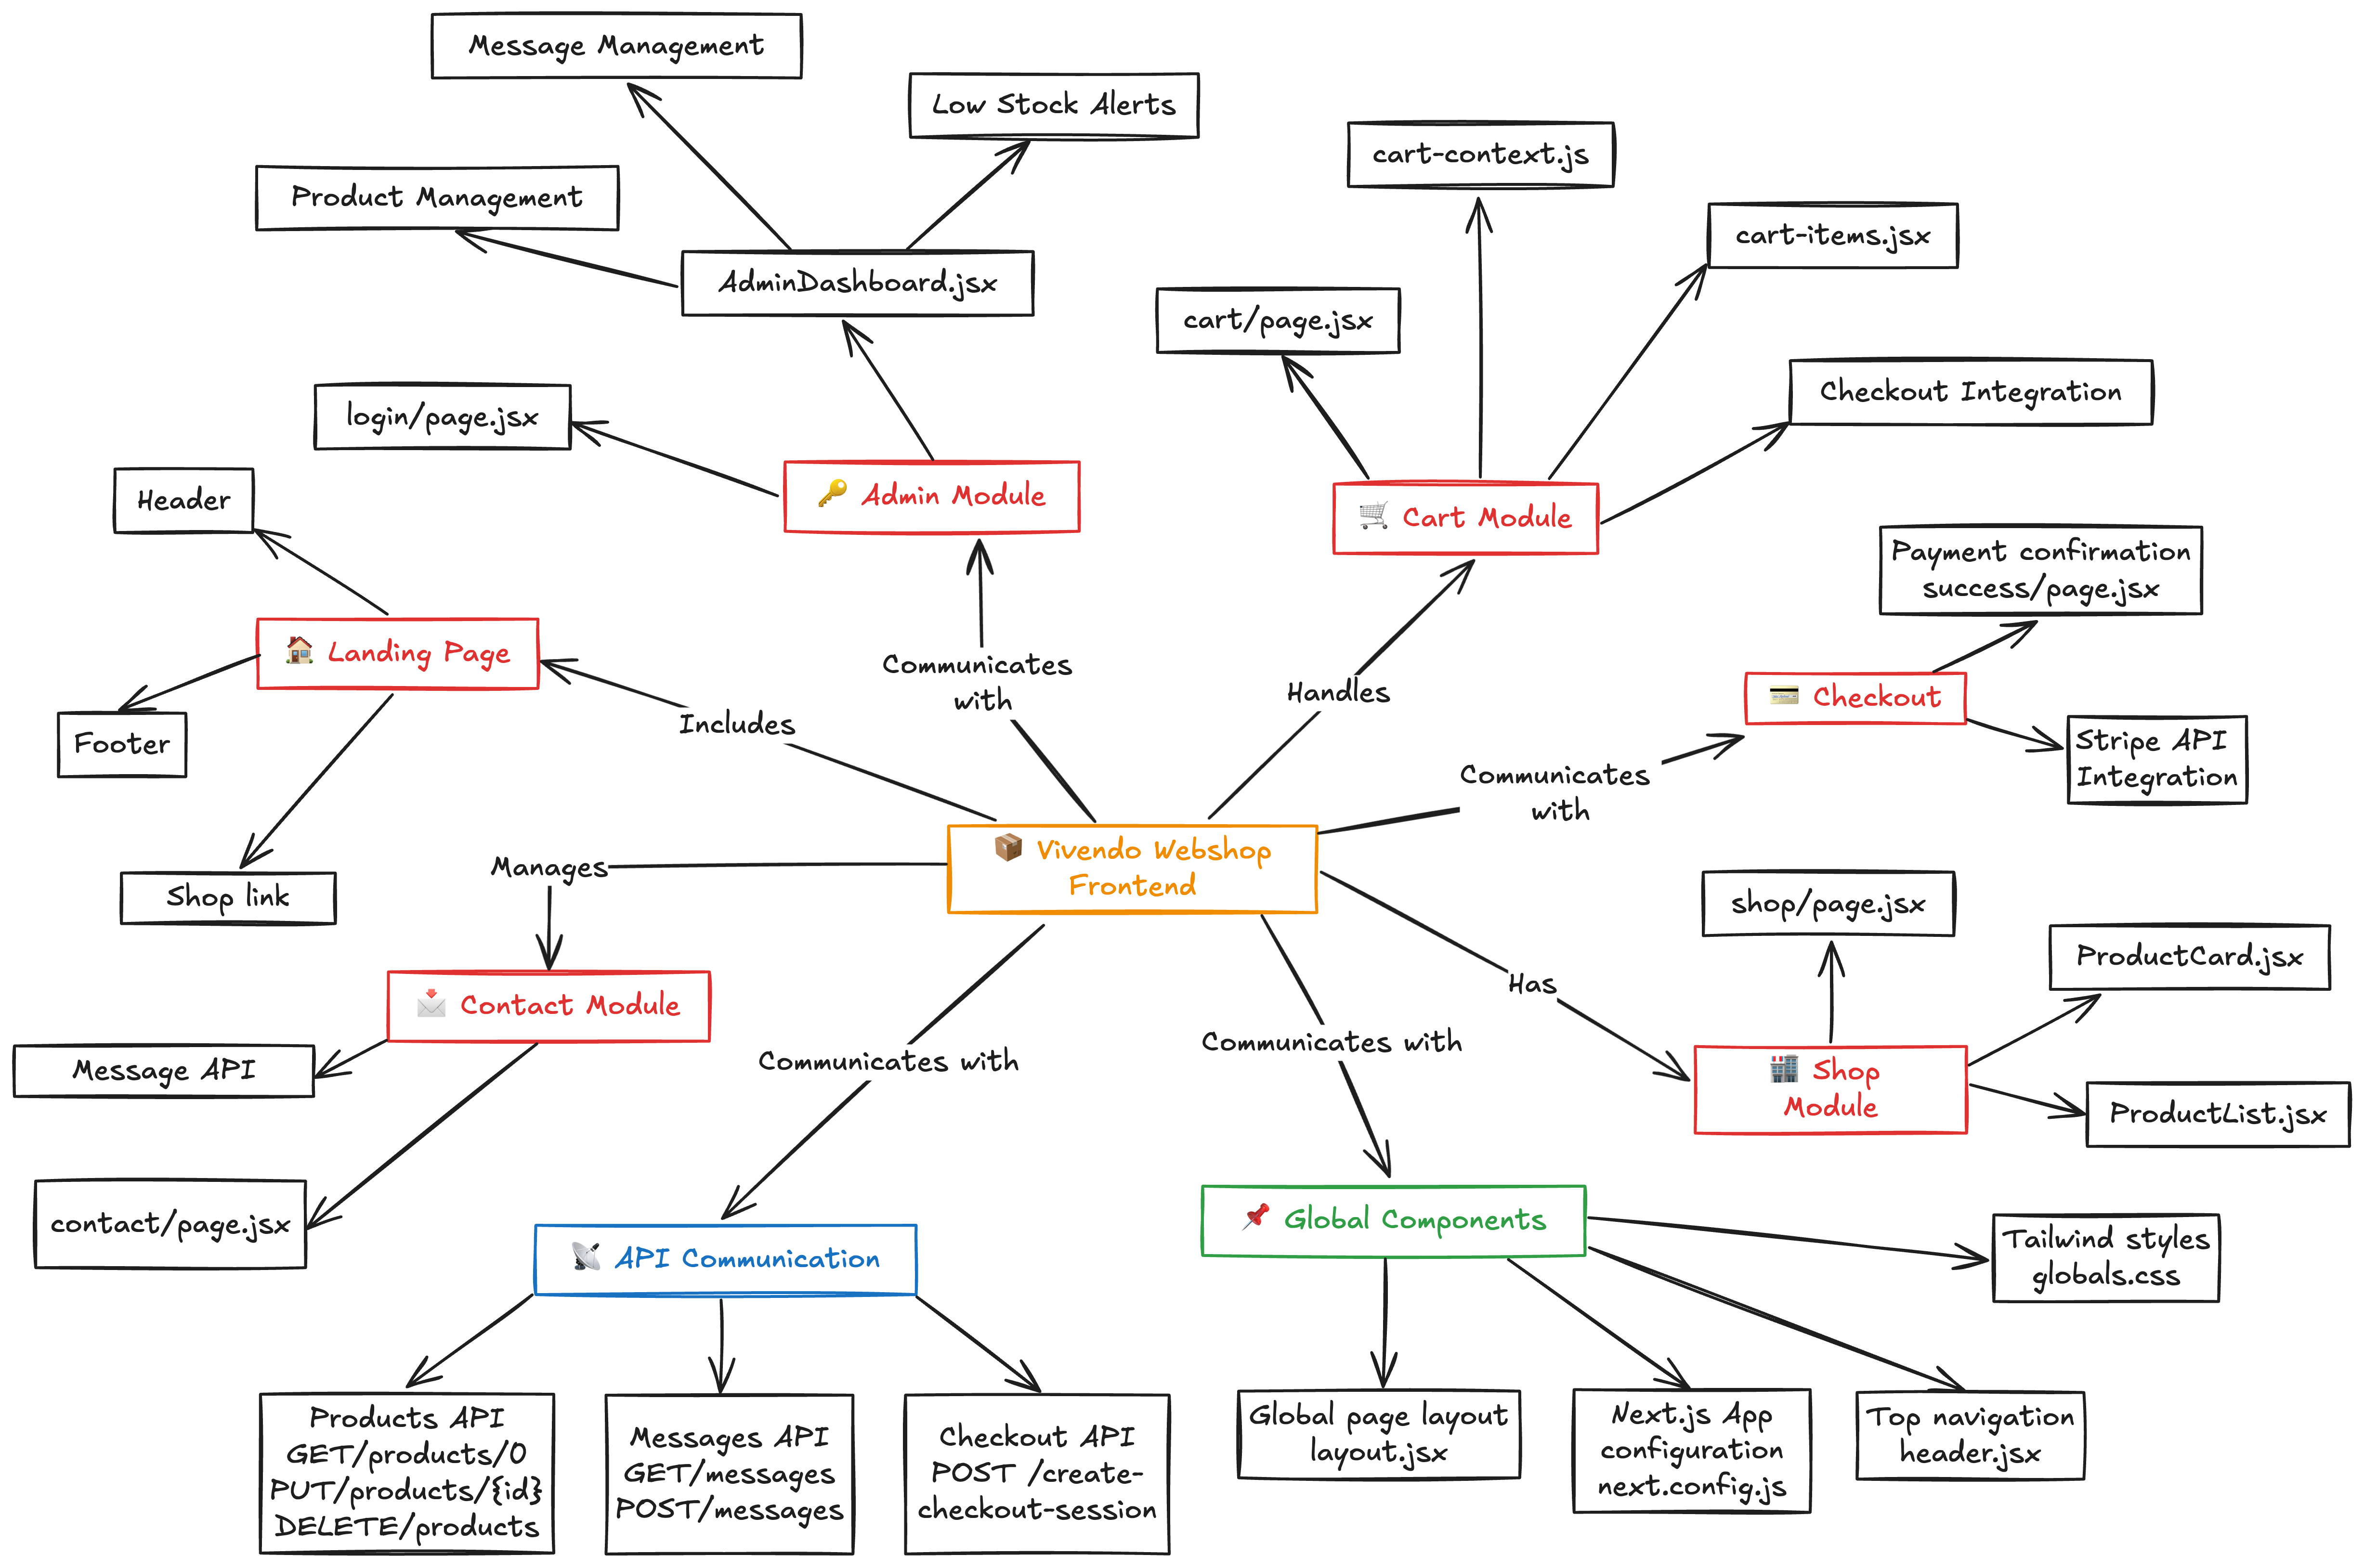
\includegraphics[width=1.3\textwidth]{images/New_frontend_architecture.png}
    }
    \caption{Component-Based Frontend Architecture}
    \label{fig:architecture}
  \end{figure}  

\subsubsection{Core Frontend Modules and Interactions}
The system consists of several modules:
\begin{itemize}
    \item \textbf{Landing Page Module}: Includes key UI components such as the header, footer and navigation links.
    \item \textbf{Admin Module}: Manages the admin dashboard, including product management, low stock alerts and message management. The admin module is responsible for managing products, messages, and stock alerts. It is connected to the \textbf{Admin Dashboard} component, which communicates with the API layer.
    \item \textbf{Cart Module}: Handles cart functionality, including cart context, cart items and checkout integration. The cart module manages cart-related functionalities and state using \texttt{cart-context.js}. It also connects with the checkout module to handle Stripe payments.
    \item \textbf{Shop Module}: Displays product listings and product cards with interactivity.
    \item \textbf{Checkout Module}: Integrates with Stripe API for handling payments and success confirmations.
    \item \textbf{Contact Module}: Manages user interactions via the contact page and handles message submissions. It connects with the API layer to store and retrieve messages.
    \item \textbf{API Communication Layer}: Manages requests to the backend services, including product APIs, messages API and checkout API. This layer serves as the middleware between the frontend and backend, making requests via REST APIs. It handles product data, message submissions, and checkout sessions.
    \item \textbf{Global Components}: Includes shared layout elements, styles and configurations.
\end{itemize}

\subsection{Backend}
\begin{figure}[!h!]
    \centering
    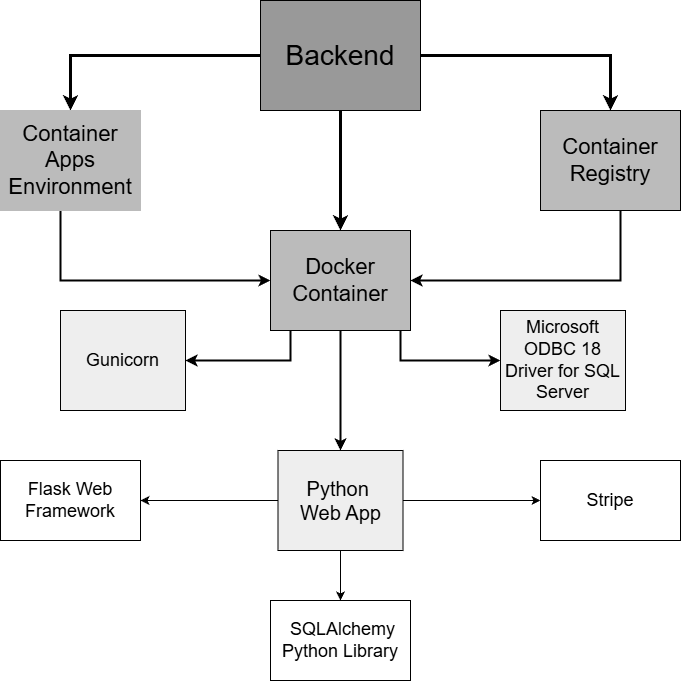
\includegraphics[width=\textwidth]{images/backend_building_block.png}
    \caption{Backend Building Block View}
    \label{fig:backend_building_block_view}
\end{figure}

The backend, whose building block view can be seen in fig. \ref{fig:backend_building_block_view}, consists of the following elements:

\begin{itemize}
    \item \textbf{Docker Container}: Runs the backend web app.
    \item \textbf{Container Registry}: Hosts the images used by the Docker container.
    \item \textbf{Container Apps Environment}: Manages the Docker container in regard to e.g., replicas and load balancing.
\end{itemize}

The Docker container consists of the following elements:

\begin{itemize}
    \item \textbf{Python Web App}: Contains all the functions of the backend.
    \item \textbf{Gunicorn}: Serves the python web app, allowing for multiple “workers”, 
    i.e., threads, making use of the multiple CPU cores available from the container app.
    \item \textbf{Microsoft ODBC 18 Driver for SQL Server}: The database driver is required in order to be able to connect to the SQL database on Azure.
\end{itemize}

The python web app consists of the following elements:

\begin{itemize}
    \item \textbf{Flask Web Framework}: Flask is a web framework for creating web applications in python.
    We use it to simplify the development of the web app in python.
    The only part the developer has to take care of, is the configuration and definition of HTTP routes.
    The other parts such as routing, parsing of request data, and listening for connections is handled by Flask.
    \item \textbf{SQLAlchemy Python Library}: The SQLAlchemy python library provides an SQL toolkit for e.g., 
    connecting to databases and configuring connection properties.
    For instance, we enable a connection pooling, which makes the backend maintain multiple connections,
    which are periodically recycled. This prevents issues with stale connections.
    \item \textbf{Stripe}: We integrate the Stripe payment processing platform, so that customers can use said platform
    to pay for products, rather than us having to deal with e.g., 
    accepting credit payments or other payment methods.
\end{itemize}

\subsection{E-Mail Service}
The Email Service is a standalone microservice designed to handle email notifications for customers in the system. Its primary task is to send confirmation emails containing the receipt in PDF format. Implemented in Python, the Email Service uses the Azure Communication Service for reliable email delivery.

The workflow starts when a customer places an order through the front-end application. The front-end submits the order details, including items, quantities, prices, and customer email, to the backend via a secure API call. The backend initiates a payment request using Stripe's Checkout API. Upon successful payment, Stripe notifies the backend via a webhook event (payment\_intent.succeeded), confirming the transaction.

After receiving and validating the Stripe webhook, the backend triggers the email service by sending a request containing the order ID and customer email. The Email Service retrieves the order details from the backend, generates a PDF receipt encapsulating the order information, and constructs an email with the PDF receipt attached. This email is then sent to the customer using the Azure Communication Service.

\subsection{Database}
We use an Azure SQL database for storing our data.
The database schema can be described with the
entity-relationship diagram seen in fig. \ref{fig:db_er_diagram}.
\begin{figure}[!h!]
    \centering
    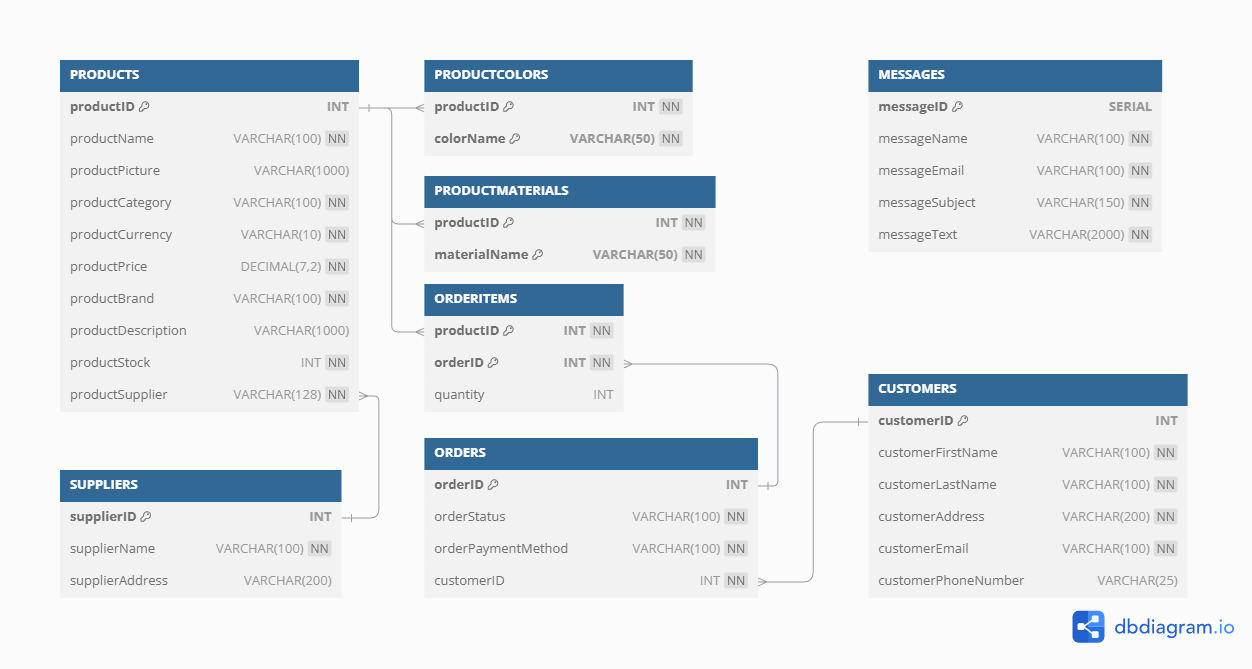
\includegraphics[width=\textwidth]{images/db_er_diagram.png}
    \caption{Database Entity-Relationship Diagram}
    \label{fig:db_er_diagram}
\end{figure}

Interaction with the database go through the SQLAlchemy ORM of the backend.

\subsection{Image Storage}
We use an Azure Storage Account as a BLOB storage for our product images.
Anonymous read requests are allowed for the product images,
allowing the frontend to fetch a product image from the BLOB storage
if it has the correct file name, 
which is included in the backend response for any given product.


\subsection{Important Interfaces}

The frontend can communicate with the backend using a RESTful API.
The following routes are used by the frontend:

\subsubsection{/product API Endpoint}

\begin{longtable}[]{@{}
    >{\raggedright\arraybackslash}p{(\columnwidth - 2\tabcolsep) * \real{0.3333}}
    >{\raggedright\arraybackslash}p{(\columnwidth - 2\tabcolsep) * \real{0.6667}}@{}}
\toprule
\begin{minipage}[b]{\linewidth}\raggedright
\textbf{Route}
\end{minipage} & \begin{minipage}[b]{\linewidth}\raggedright
\textbf{Methods}
\end{minipage} \\
\midrule
\endhead
\begin{itemize}
    \item /products
    \item /products/<ID>
\end{itemize} &
\begin{itemize}
  \item GET
  \item POST
  \item PUT
  \item DELETE
\end{itemize} \\
\bottomrule
\end{longtable}

This route concerns itself with products. The admin panel has access to POST, PUT, and DELETE operations, 
while the webshop only has access to GET. GET returns a JSON object containing information about
the product with the given ID.
The object contains the following fields:
\begin{itemize}
    \item \textit{id}: Identifier for the product
    \item \textit{name}: Name of the product. Example: “Modern Sofa”.
    \item \textit{category}: Category of the product. Example: “Sofas”.
    \item \textit{price}: Unit price of the product. Example: “999.99”.
    \item \textit{currency}: Currency symbol. Example: “€”.
    \item \textit{description}: Detailed description of the product. Example: “A sleek and luxurious sofa that \dots”.
    \item \textit{brand}: Brand producing the product. Example: “Furniture LLC”.
    \item \textit{materials}: A list of materials the product is made out of. Example: “[Fabric]”.
    \item \textit{colors}: A list of colors of the product. Example: “[gray]”.
    \item \textit{pictureUrl}: The file name under which our BLOB storage stores the product image. Example: “modern-sofa.webp”.
\end{itemize}
There is no product with an ID of 0. Instead, inputting ID 0 retrieves all the products in the shop catalog
as a list of JSON objects.

\subsubsection{/messages API Endpoint}

\begin{longtable}[]{@{}
    >{\raggedright\arraybackslash}p{(\columnwidth - 2\tabcolsep) * \real{0.3333}}
    >{\raggedright\arraybackslash}p{(\columnwidth - 2\tabcolsep) * \real{0.6667}}@{}}
\toprule
\begin{minipage}[b]{\linewidth}\raggedright
\textbf{Route}
\end{minipage} & \begin{minipage}[b]{\linewidth}\raggedright
\textbf{Methods}
\end{minipage} \\
\midrule
\endhead
\begin{itemize}
    \item /messages
    \item /messages/<ID>
\end{itemize} &
\begin{itemize}
    \item GET
    \item POST
    \item DELETE
\end{itemize} \\
\bottomrule
\end{longtable}

This endpoint is responsible for handling messages that customers can leave if they have questions or any other issues. Customers can submit their messages through a POST request on the contact page of the website. Once submitted, the admin can view all the messages via a GET request. Both the GET and POST requests follow a similar JSON structure, which includes the following fields:

\begin{itemize}
    \item \textit{id}: Identifier for the message (only accessible for GET request. POST requests add a new message to the database, hence the id is created at that point).
    \item \textit{name}: Name of the person who wants to get in contact with the vivendo staff.
    \item \textit{email}: E-Mail address of that person, so that the admin can answer the request of the person.
    \item \textit{subject}: A title for the request.
    \item \textit{message}: The request the person has. This field can have up to 1000 characters.
\end{itemize}

Unlike the product endpoint, the message endpoint does not require an ID when retrieving all messages via a GET request. This is because the admin can simply view all messages without the need for any specific identifier. However, an ID is required when the admin wants to delete a particular message using a DELETE request. The ID ensures that the correct message is deleted from the database, allowing for accurate and targeted operations.

\subsubsection{/create-checkout-session API Endpoint}

The \texttt{/create-checkout-session} API endpoint is the backend's entry point for initiating the payment process, facilitating the transition from a customer's cart submission to Stripe's hosted checkout experience. It handles the creation of a Stripe Checkout session and ensures order details are persisted for downstream processing.

\begin{longtable}[]{@{}
    >{\raggedright\arraybackslash}p{(\columnwidth - 2\tabcolsep) * \real{0.3333}}
    >{\raggedright\arraybackslash}p{(\columnwidth - 2\tabcolsep) * \real{0.6667}}@{}}
\toprule
\begin{minipage}[b]{\linewidth}\raggedright
\textbf{Route}
\end{minipage} & \begin{minipage}[b]{\linewidth}\raggedright
\textbf{Methods}
\end{minipage} \\
\midrule
\endhead
\begin{itemize}\itemsep0em
    \item \texttt{/create-checkout-session}
\end{itemize} &
\begin{itemize}\itemsep0em
    \item \texttt{POST}
\end{itemize} \\
\bottomrule
\end{longtable}

The endpoint accepts POST requests from the frontend, which submits a JSON payload containing the cart details such as item names, quantities, prices, and the customer's email. Upon receiving the request, the backend performs the following steps:
\begin{enumerate}
    \item \textbf{Validation:} Ensures required fields (e.g., items and email) are present and valid. If not, it returns a \texttt{400 Bad Request} response with an error message.
    \item \textbf{Stripe Session Creation:} Constructs a Stripe Checkout session using the Stripe API. Cart items are transformed into line items, with prices converted to cents and the currency set to EUR. Success and cancel URLs are dynamically generated from the request's origin (e.g., \texttt{http://frontend-domain/success}), and metadata including the \texttt{order\_id} is attached. The customer's email is also embedded for receipt purposes.
    \item \textbf{Response:} Returns a \texttt{200 OK} response with the Stripe session ID, which the frontend uses to redirect the customer to Stripe's checkout page. If an error occurs (e.g., Stripe API failure), it rolls back the database transaction and returns a \texttt{500 Internal Server Error}.
\end{enumerate}

Once the session ID is received, the frontend leverages the \texttt{Stripe.js} library to redirect the customer to Stripe's hosted checkout page, where payment is completed. The endpoint's role concludes here, with payment confirmation handled asynchronously via the \texttt{/webhook} endpoint.

\subsubsection{/webhook API Endpoint}

The \texttt{/webhook} API endpoint enables the backend to receive asynchronous event notifications from Stripe, facilitating real-time processing of payment outcomes. It serves as the critical link between Stripe’s payment system and the backend’s notification workflows.

\begin{longtable}[]{@{}
    >{\raggedright\arraybackslash}p{(\columnwidth - 2\tabcolsep) * \real{0.3333}}
    >{\raggedright\arraybackslash}p{(\columnwidth - 2\tabcolsep) * \real{0.6667}}@{}}
    \toprule
    \begin{minipage}[b]{\linewidth}\raggedright
    \textbf{Route}
    \end{minipage} & \begin{minipage}[b]{\linewidth}\raggedright
    \textbf{Methods}
    \end{minipage} \\
    \midrule
    \endhead
    \begin{itemize}
        \item \texttt{/webhook}
    \end{itemize} &
    \begin{itemize}
        \item \texttt{POST}
    \end{itemize} \\
    \bottomrule
\end{longtable}

The endpoint processes POST requests from Stripe, which delivers event data in JSON format whenever a payment-related action occurs, such as the \texttt{payment\_intent.succeeded} event indicating a successful transaction. The backend handles these requests as follows:
\begin{enumerate}
    \item \textbf{Validation:} Verifies the request’s authenticity by checking the \texttt{Stripe-Signature} header against the \texttt{STRIPE\_WEBHOOK\_SECRET} environment variable. If invalid, it returns a \texttt{400 Bad Request} response.
    \item \textbf{Event Processing:} Extracts essential data from the payload, including the payment intent ID, amount received (in cents), customer email, and metadata (e.g., \texttt{order\_id}). 
    \item \textbf{Notification Trigger:} Initiates the Email Service by dispatching a request with the \texttt{order\_id} and customer email, then returns a \texttt{200 OK} response to Stripe.
\end{enumerate}

This interface ensures secure and reliable communication with Stripe, leveraging the webhook’s event-driven nature to synchronize payment status with backend operations.

